	\subsection{Percorrenza di un Treno}
	
	A ciascuna entità Treno, è assegnato un Percorso (\ttt{Route}) che comprende andata e ritorno, composto da una sequenze di Tappe (\ttt{Stage}) successive, ciascuna contenente i seguenti campi:
				\begin{center}
\begin{verbatim}
    - start_station,
    - start_platform,
    - next_segment,
    - next_station,
    - next_platfom,
    - leave_action,
    - enter_action,
    - node_name
\end{verbatim}
				\end{center}
dove \ttt{leave\_action} e \ttt{enter\_action} indicano rispettivamente quello che un Treno dovrà compiere alla partenza dalla stazione \ttt{start\_station} e all'arrivo presso la prossima stazione \ttt{next\_station}, a scelta tra \ttt{ENTER}, per entrare ed effettuare discesa e salita passeggeri o \ttt{PASS} per non fermarsi e oltrepassare la Stazione; il campo \ttt{node\_name} invece, indica la regione di destinazione, e viene utilizzato nel caso di transito su stazione di Gateway.
	Il percorso di ciascun Treno è scandito da una Tabella degli Orari (\ttt{Time\_Table}), la quale definisce per $N>1$ Corse (\ttt{Runs}) successive del Percorso, gli \ii{orari di partenza} dalle Stazioni da rispettare per ciascuna Tappa. 
	 
Una volta che un thread del pool della struttura \ttt{Train\_Pool} ottiene un Descrittore, effettua le seguenti  operazioni, per ciascuna Tappa del Percorso corrente (di andata o di ritorno):
				\begin{itemize} 
					\item Partenza dalla Stazione \ttt{start\_station}, Piattaforma \ttt{start\_platfom} all'orario indicato da \ttt{Time\_Table} per la Tappa corrente; se previsto (\ttt{action = ENTER}) allora effettua la salita dei Viaggiatori.
					\item Accesso al prossimo Segmento \ttt{next\_segment}.
					\item Percorrenza all'interno del Segmento come attesa finita di durata proporzionale alla lunghezza del Segmento e alla velocità massima alla quale il Treno può percorrerlo.
					\item Uscita dal Segmento e richiesta di Accesso alla Stazione successiva (\ttt{next\_station}) presso la Piattaforma indicata da \ttt{next\_platfom}, per eseguire l'azione \ttt{action}.
					\item Se \ttt{action = ENTER} allora effettua discesa Viaggiatori in attesa dell'arrivo del Treno.
					\item Se ci sono ancora Tappe da percorrere nel percorso (\ttt{Route}), allora il l'indice della prossima tappa del Descrittore del Treno corrente viene incrementato, e lo stesso Descrittore viene inserito in una delle code di \ttt{Train\_Pool} (in base alla priorità). 
				\end{itemize}


% ############################################################################################################
% ################################################ DEFINIZIONE_ORARI #########################################
% ############################################################################################################

		\subsubsection{Gestione della Tabella degli Orari}
		
		Per limitare la dimensione della Tabella degli Orari per ciascun percorso, esso mantiene un numero $N$ di corse. Essa viene fornita dalla Biglietteria Centrale, la quale dovrà essere sempre aggiornata relativamente alla corsa correntemente percorsa da un Treno per poter permettere la prenotazione dei Biglietti per Treni di tipo \ttt{FB} (si veda il paragrafo \ref{subsubsec:validation}). Per poter consultare la \ttt{Time\_Table}, vengono quindi utilizzati due indici:
		
		\begin{itemize}
			\item \ttt{Current\_Run} che mantiene l'indice della Corsa corrente.
			\item \ttt{Current\_Stage} che serve ad accedere l'orario per la tappa successiva.
		\end{itemize}
		
	Tali indici vengono aggiornati dal Treno al momento della partenza da una Stazione per raggiungere la Tappa successiva. Nel caso in cui il Treno ultimi una corsa, esso incrementa l'indice \ttt{Current\_Run}, ed invia un messaggio remoto \ii{sincrono} alla Biglietteria Centrale comunicando il passaggio alla Corsa successiva. Ci sono due possibili risultati alla richiesta di aggiornamento:
	\begin{itemize}
		\item Si è raggiunta l'ultima Corsa ($N-esima$), e quindi viene restituita una nuova \ttt{Time\_Table} contenente gli orari per $N$ corse, composta dalla corsa $N-esima$ della Tabella precedente in prima posizione, e da $N-1$ Corse calcolate. L'indice \ttt{Current\_Run} viene posto ad 1, e viene memorizzato l'identificativo della Corsa corrente \ttt{Current\_Run\_Id}, il quale può essere ad esempio, un numero progressivo che la identifica.
		\item Non si è raggiunta l'ultima corsa, e quindi viene aggiornata la corsa corrente presso la Biglietteria Centrale e restituito l'identificativo della stessa.
	\end{itemize}
	
	La scelta di riportare solo l'orario di partenza nella definizione della Tabella degli orari, permette di risolvere i problemi causati dal passaggio di alcuni Treni attraverso Regioni su nodi distribuiti, dovuti, ad esempio, dai clock non sincronizzati dei nodi di calcolo che compongono il sistema, o dai ritardi che possono essere introdotti dalla trasmissione sulla rete. Si supponga una differenza in valore assoluto $\Delta t$ tra i clock $t_1$ e $t_2$ di due Nodi $N_1$ ed $N_2$, e supponiamo di avere un treno $T$ che viaggia da $N_1$ ad $N_2$. Si presentano i seguenti due casi:
	
	\begin{itemize}
		\item $t_1 = t_2+\Delta t$: il Treno $T$ localmente ad $N_2$ potrà avere un ritardo aggiuntivo compreso tra $0$ e $\Delta t$ rispetto all'eventuale ritardo accumulato in $N_1$;
		\item $t_2 = t_1+\Delta t$: il Treno $T$ si ritroverà in anticipo rispetto al clock di $N_1$, e quindi vi è la possibilità che prolunghi la sua attesa.
	\end{itemize}
	
	
% ############################################################################################################
% ################################################# ACCESSO_SEGMENTO #########################################
% ############################################################################################################
	
		\subsubsection{Accesso ad un Segmento}\label{subsubsec:segment_access}
		
		L'accesso alla risorsa protetta Segmento è regolato da una interfaccia ben definita, che permette:
			\begin{itemize}
				\item Ingresso.
				\item Uscita.
			\end{itemize}
		Per mantenere l'ordine di accesso, ciascun Segmento \ttt{Segment} è dotato di una Coda FIFO (\ttt{Train\_Queue}) che conterrà i Descrittori dei Treni correntemente in transito.		
		\begin{description}
			
			\item {\ii{Ingresso}}
			
			La richiesta di accesso (\ttt{Enter}) al segmento avviene in mutua esclusione tra tutti le entità Treno. In ogni momento quindi solo una entità eseguirà all'interno della risorsa protetta. Supponendo la presenza di un flag booleano \ttt{Free} che permette di indicare lo stato occupato della risorsa, una volta ottenuta la risorsa ciascun Treno compie le seguenti operazioni:
			 \begin{itemize}
			 	\item Se \ttt{Free=False} e la direzione di percorrenza corrente è opposto a quella del Treno che vuole accedere, allora il thread corrente si pone in attesa sulla condizione \ttt{wait(Not\_Free)}
			 	\item Inserimento del Descrittore nella coda \ttt{Train\_Queue};
			 	\item Aggiornamento della velocità di percorrenza del Treno entrato, in base a quella dei Treni che lo precedono.
			 	\item Nel caso in cui la risorsa risulti vuota (\ttt{Free=True}), allora viene modificato il valore di \ttt{Free} a \ttt{False} , e memorizzata la stazione di provenienza del Treno.
			\end{itemize}
			
			Una volta terminate queste operazioni, il thread rappresentante il Treno rilascia la risorsa e, basandosi sulla lunghezza del Segmento e sulla velocità da mantenere, simula la percorrenza rendendosi inattivo (non competitivo per l'ottenimento della CPU) per un tempo dato dalla semplice equazione: $ Time = Segment\_Length / Actual\_Speed $.
			
			Data la possibilità di percorrenza multipla del Segmento, si presentano diverse problematiche: per la semantica descritta,  nel caso in cui una volta ottenuta la possibilità di eseguire all'interno della procedura protetta per l'accesso al Segmento, un Treno richieda l'accesso nella direzione opposta a quella dei Treni che percorrono il Segmento (ovvero abbiamo la situazione in cui il flag booleano \ttt{Free = False}, e la stazione di provenienza memorizzata presso il Segmento è diversa da quella del Treno richiedente) allora questo dovrà attendere  fino a che il Segmento non si sarà liberato dai Treni in transito. Questa attesa dev'essere tale da evitare starvation del Treno in attesa.
			
			Una primo approccio possibile per evitare questo problema è garantire ai Treni in attesa su condizione una priorità maggiore nell'accedere al Segmento appena esso diviene libero rispetto ad altri Treni che sopraggiungono successivamente. Per questo possiamo utilizzare due variabili di condizione distinte per porre i thread in attesa, una per ciascuno dei due estremi del Segmento : \ttt{Can\_Enter\_First\_End} e \ttt{Can\_Enter\_Second\_End}.
			
			Questi accorgimenti non risultano però sufficiente a garantire che i Treni in attesa avranno accesso al Segmento in qualche momento: si consideri, ad esempio, la presenza di un percorso circolare composto da $N$ Segmenti, e di $M$ Treni che viaggiano lungo tale percorso in senso orario in modo tale che in ogni istante ci sia almeno un treno all'interno di ciascun Segmento. Se ora aggiungiamo al sistema un Treno che viaggia in direzione opposta, allora esso, adottando la semantica di accesso descritta, non riuscirà mai a percorrere uno dei Segmenti.			
			
			Una possibile soluzione a questo problema, è prevedere un \ii{numero massimo di accessi consecutivi per direzione}. Un thread viene posto in attesa sulla variabile di condizione presso la quale si vuole effettuare l'accesso, se il numero massimo di accessi da una direzione è stato raggiunto. 
		Sia \ttt{Access\_Number} il numero di accessi nella direzione corrente, e sia \ttt{Current\_Direction} la direzione di percorrenza corrente, che indica l'accesso da uno dei due estremi del Segmento.
		
		La semantica adottata per la regolazione dell'accesso è la seguente:
		\begin{itemize}
			\item Sia $T$ il thread Treno che esegue correntemente. Esso potrà accedere al segmento se e soltanto se una delle seguenti condizioni è verificata:
				\begin{itemize}
					\item \ttt{Free = True}
					\item \ttt{Free = False}, \ttt{Current\_Direction} coincide con l'estremo dal quale accede $T$ ma il numero massimo di accessi per direzione non è stato raggiunto.
					\item \ttt{Free = False}, \ttt{Current\_Direction} coincide con l'estremo dal quale accede $T$, e il numero massimo di accessi per direzione è stato raggiunto ma il numero di Treni in attesa di accedere in direzione opposta è 0.
				\end{itemize}
			\item Se $T$ non può accedere, allora a seconda della direzione con la quale intende percorrere il Segmento, viene posto in attesa su condizione \ttt{Can\_Enter\_First\_End} oppure \ttt{Can\_Enter\_Second\_End} con una \ttt{wait}. Una possibile realizzazione in pseudo-codice del controllo può essere:
\begin{lstlisting}
monitor Segment_Monitor
	...
	procedure Enter(T:Train,Access_End:integer) 
	begin
		...
		while(Can_Not_Access) loop
			if Access_End = First_End then
				wait(Can_Enter_First_Edge);
			else
				wait(Can_Enter_Second_Edge);
			end if;
		end loop;
	...
\end{lstlisting}
			\item Una volta che $T$ ha ottenuto l'accesso:
				\begin{itemize}
					\item Se \ttt{Free = True} allora occupa il Segmento (imposta \ttt{Free} a \ttt{False}) e assegna a \ttt{Access\_Number} il valore $1$, se la direzione di $T$ è diversa da quella corrente memorizzata nel Segmento;
					\item Altrimenti, incrementa di $1$ il valore di \ttt{Access\_Number} se esso è inferiore al limite massimo consentito.
					\item In ciascuno dei due casi infine, inserisce il Descrittore del Treno nella coda \ttt{Train\_Queue} e aggiorna la Velocità di percorrenza.
				\end{itemize}
		\end{itemize}
			
			Una volta che il Segmento si sarà liberato (\ttt{Free=True}) allora ciascun Treno in attesa nella coda relativa all'estremità opposta a quella di accesso dell'ultimo Treno uscito, potrà ritentare l'accesso al Segmento (la coda viene svuotata e ripopolata).
			Si noti che la soluzione presentata non garantisce accesso preferenziale ai treni di tipo FB, requisito desiderabile. Per introdurre priorità senza poter fare assunzioni sulle politiche di scheduling che verranno utilizzate è possibile procedere nel seguente modo: viene introdotta una nuova risorsa protetta da monitor, \ttt{Priority\_Access\_Handler}, la quale mantiene due variabili intere \ttt{FB\_Count} e \ttt{Regional\_Count}, un flag booleano \ttt{Free} e due varibili di condizione \ttt{Can\_Access\_FB} e \ttt{Can\_Access\_Regional}. Tale risorsa avrà la seguente semantica in pseudo-codice:
	
\begin{lstlisting}[caption=Typo monitor utilizzato per garantire accesso preferenziale a Treni di tipo FB,label=priority_access_controller]
monitor Priority_Access_Handler 
	...
	procedure Gain_Access(T:Train) 
	begin
		if not Free then
			if T.Type = FB then
				FB_Count := FB_Count + 1;
				wait(Can_Access_FB);
				FB_Count := FB_Count - 1;
			else
				Regional_Count := Regional_Count + 1;
				wait(Can_Access_Regional);
				Regional_Count := Regional_Count - 1;
			end if;
		end if;
		Free := False;
	end;
	
	procedure Access_Gained()
	begin
		Free := True;
		if FB_Count > 0 then
			signal(Can_Access_FB);
		else
			signal(Can_Access_Regional);
		end if;
	end;
end monitor;
\end{lstlisting}
			
			Questa struttura può essere utilizzata nel modo seguente: supponiamo di avere una struttura dati contenente un oggetto \ttt{Priority\_Access\_Handler} e un oggetto \ttt{Segment}, la quale espone una interfaccia composta da \ttt{Add\_Train}, procedura che aggiunge un dato Descrittore di Treno in una coda interna \ttt{Trains\_Order} che specifica l'ordine di accesso, e da \ttt{Enter} e \ttt{Leave} rispettivamente per entrare ed uscire dal Segmento. \ttt{Enter} può avere il seguente comportamento:
			
\begin{lstlisting}
	
...
// procedura non thread safe
procedure Enter(Train:Train,Segment:Segment) is
begin
	// Se l'oggetto Priority_Controller e' libero, 
	// viene occupato e si procede oltre, altrimenti 
	// il thread corrente si trovera' in attesa su  
	// variabile di condizione Can_Access_FB o 
	// Can_Access_Regional.
	Segment.Priority_Controller.Gain_Access(Train);
	// A questo punto il thread corrente e' l'unico  
	// in esecuzione e quindi puo' inserire il  
	// descrittore nella coda interna a Segment_Monitor. 
	// Nel frattempo altri thread possono attendere
	// nelle code di attesa di Priority_Controller.
	Segment.Segment_Monitor.Add_Train(Train);
	// Una volta eseguito l'operazione Add_Train si 
	// puo' liberare l'Access_Controller
	Segment.Priority_Controller.Access_Gained();
	// A questo punto viene fatta la richiesta 
	// di Accesso. Anche in caso di prerilascio, 
	// esso verra' attuato secondo l'ordine 
	// descritto nella coda interna Trains_Order.
	Segment.Segment_Monitor.Enter(Train);
end;
	
\end{lstlisting}

	mentre \ttt{Leave} semplicemente invoca \ttt{Leave} su \ttt{Segment}. La semantica di accesso ordinato in base al contenuto della coda \ttt{Trains\_Order} è il seguente:
	
\begin{lstlisting}

monitor Segment_Monitor
	...
	procedure Enter(T : Train) 
	begin
		
		// Se il Treno corrente T non e' il
		// prossimo designato, attende.
		while(Trains_Order.First_Element() /= T) loop
			wait(Not_First);
		end loop;
		
		Trains_Order.Dequeue(T1);
		
		// Invoca una signal su variabile di 
		// condizione, risvegliando in maniera
		// ordinata i thread in attesa.
		// Fino a quando il thread corrente non
		// abbandonera' la risorsa (ovvero 
		// terminera' l'esecuzione della procedura
		// corrente) essi non potranno eseguire.
		signal_all(Not_First);
		
		// Procedi con l'accesso secondo la 
		// semantica desctitta
		...
	end;

end monitor;	
	
\end{lstlisting}
			
			Sebbene questo meccanismo introduca una maggiore complessità anche in termini computazionali, esso garantisce un certo livello di priorità nell'accedere al Segmento per i Treni di tipo \ttt{FB}.
			
			Per semplicità, si può assumere che vi sia uno spazio apposito dove i Treni possano attendere affinché si liberi il Segmento.
			  
			\item {\ii{Uscita}}
			
			L'uscita (\ttt{Leave}) da una Segmento da parte di una entità Treno, ha come prerequisito l'aver avuto accesso al Segmento. \'E quindi possibile assumere che il descrittore del Treno che intende uscire dal Segmento sia presente all'interno della coda \ttt{Train\_Queue}, e che inoltre al momento di tale richiesta abbia già terminato il tempo previsto di attesa che simula la percorrenza.
			
			Il requisito principale richiesto dall'azione di uscita è che essa avvenga in \ii{maniera ordinata}, in base all'ordine con cui i Treni hanno avuto accesso al Segmento. La soluzione apportata mira a garantire tale ordine di uscita, senza fare alcuna assunzione sull'ordine con il quale i Treni verranno scelti per l'esecuzione dallo scheduler. La semantica adottata è quindi la seguente:
			\begin{itemize}
				 \item Viene controllato per prima cosa se il Treno corrente è effettivamente il prossimo che deve uscire secondo l'ordine di ingresso stabilito da \ttt{Train\_Queue}.
				 \item Se è il prossimo (vengono confrontati i Descrittori), allora il Treno può abbandonare la risorsa protetta, e di conseguenza viene rimosso dalla coda \ttt{Train\_Queue}. 
				 \begin{itemize}
				 	\item Nel caso in cui il Treno corrente fosse l'ultimo in transito, allora viene posto \ttt{Free=True} e, nel caso vi siano thread in attesa presso la variabile di condizione relativa alla direzione opposta a quella del Treno uscito, allora viene effettuata una \ttt{signal} su di essa per ciascun thread in attesa. 
				 	\item Se il Treno corrente non era l'ultimo, allora invoca una \ttt{signal} sulla guardia booleana \ttt{Can\_Retry\_Exit} per ciascun thread in attesa.
				 \end{itemize}
				 \item Altrimenti il thread relativo al Treno corrente viene posto in attesa sulla condizione di uscita \ttt{Can\_Retry\_Exit}. Una volta risvegliato da una \ttt{signal}, se il Treno con thread correntemente in esecuzione non è il prossimo Treno destinato ad uscire, esso verrà posto nuovamente in attesa su \ttt{Can\_Retry\_Exit}. 
			\end{itemize}
		\end {description}
	
	La semantica descritta, garantisce ingresso sequenziale a molteplicità limitata, e uscita ordinata secondo l'ordine di ingresso. Il passo successivo consiste nel garantire l'accesso alla Stazione con lo stesso ordine di uscita per tutti i Treni provenienti dallo stesso Segmento.

% ############################################################################################################
% ####################################### ACCESSO_STAZIONE_REGIONALE #########################################
% ############################################################################################################

		\subsubsection{Accesso ad una Stazione Regionale}\label{subsubsec:regional_station_access}
		
		\begin{figure}[htbp]
			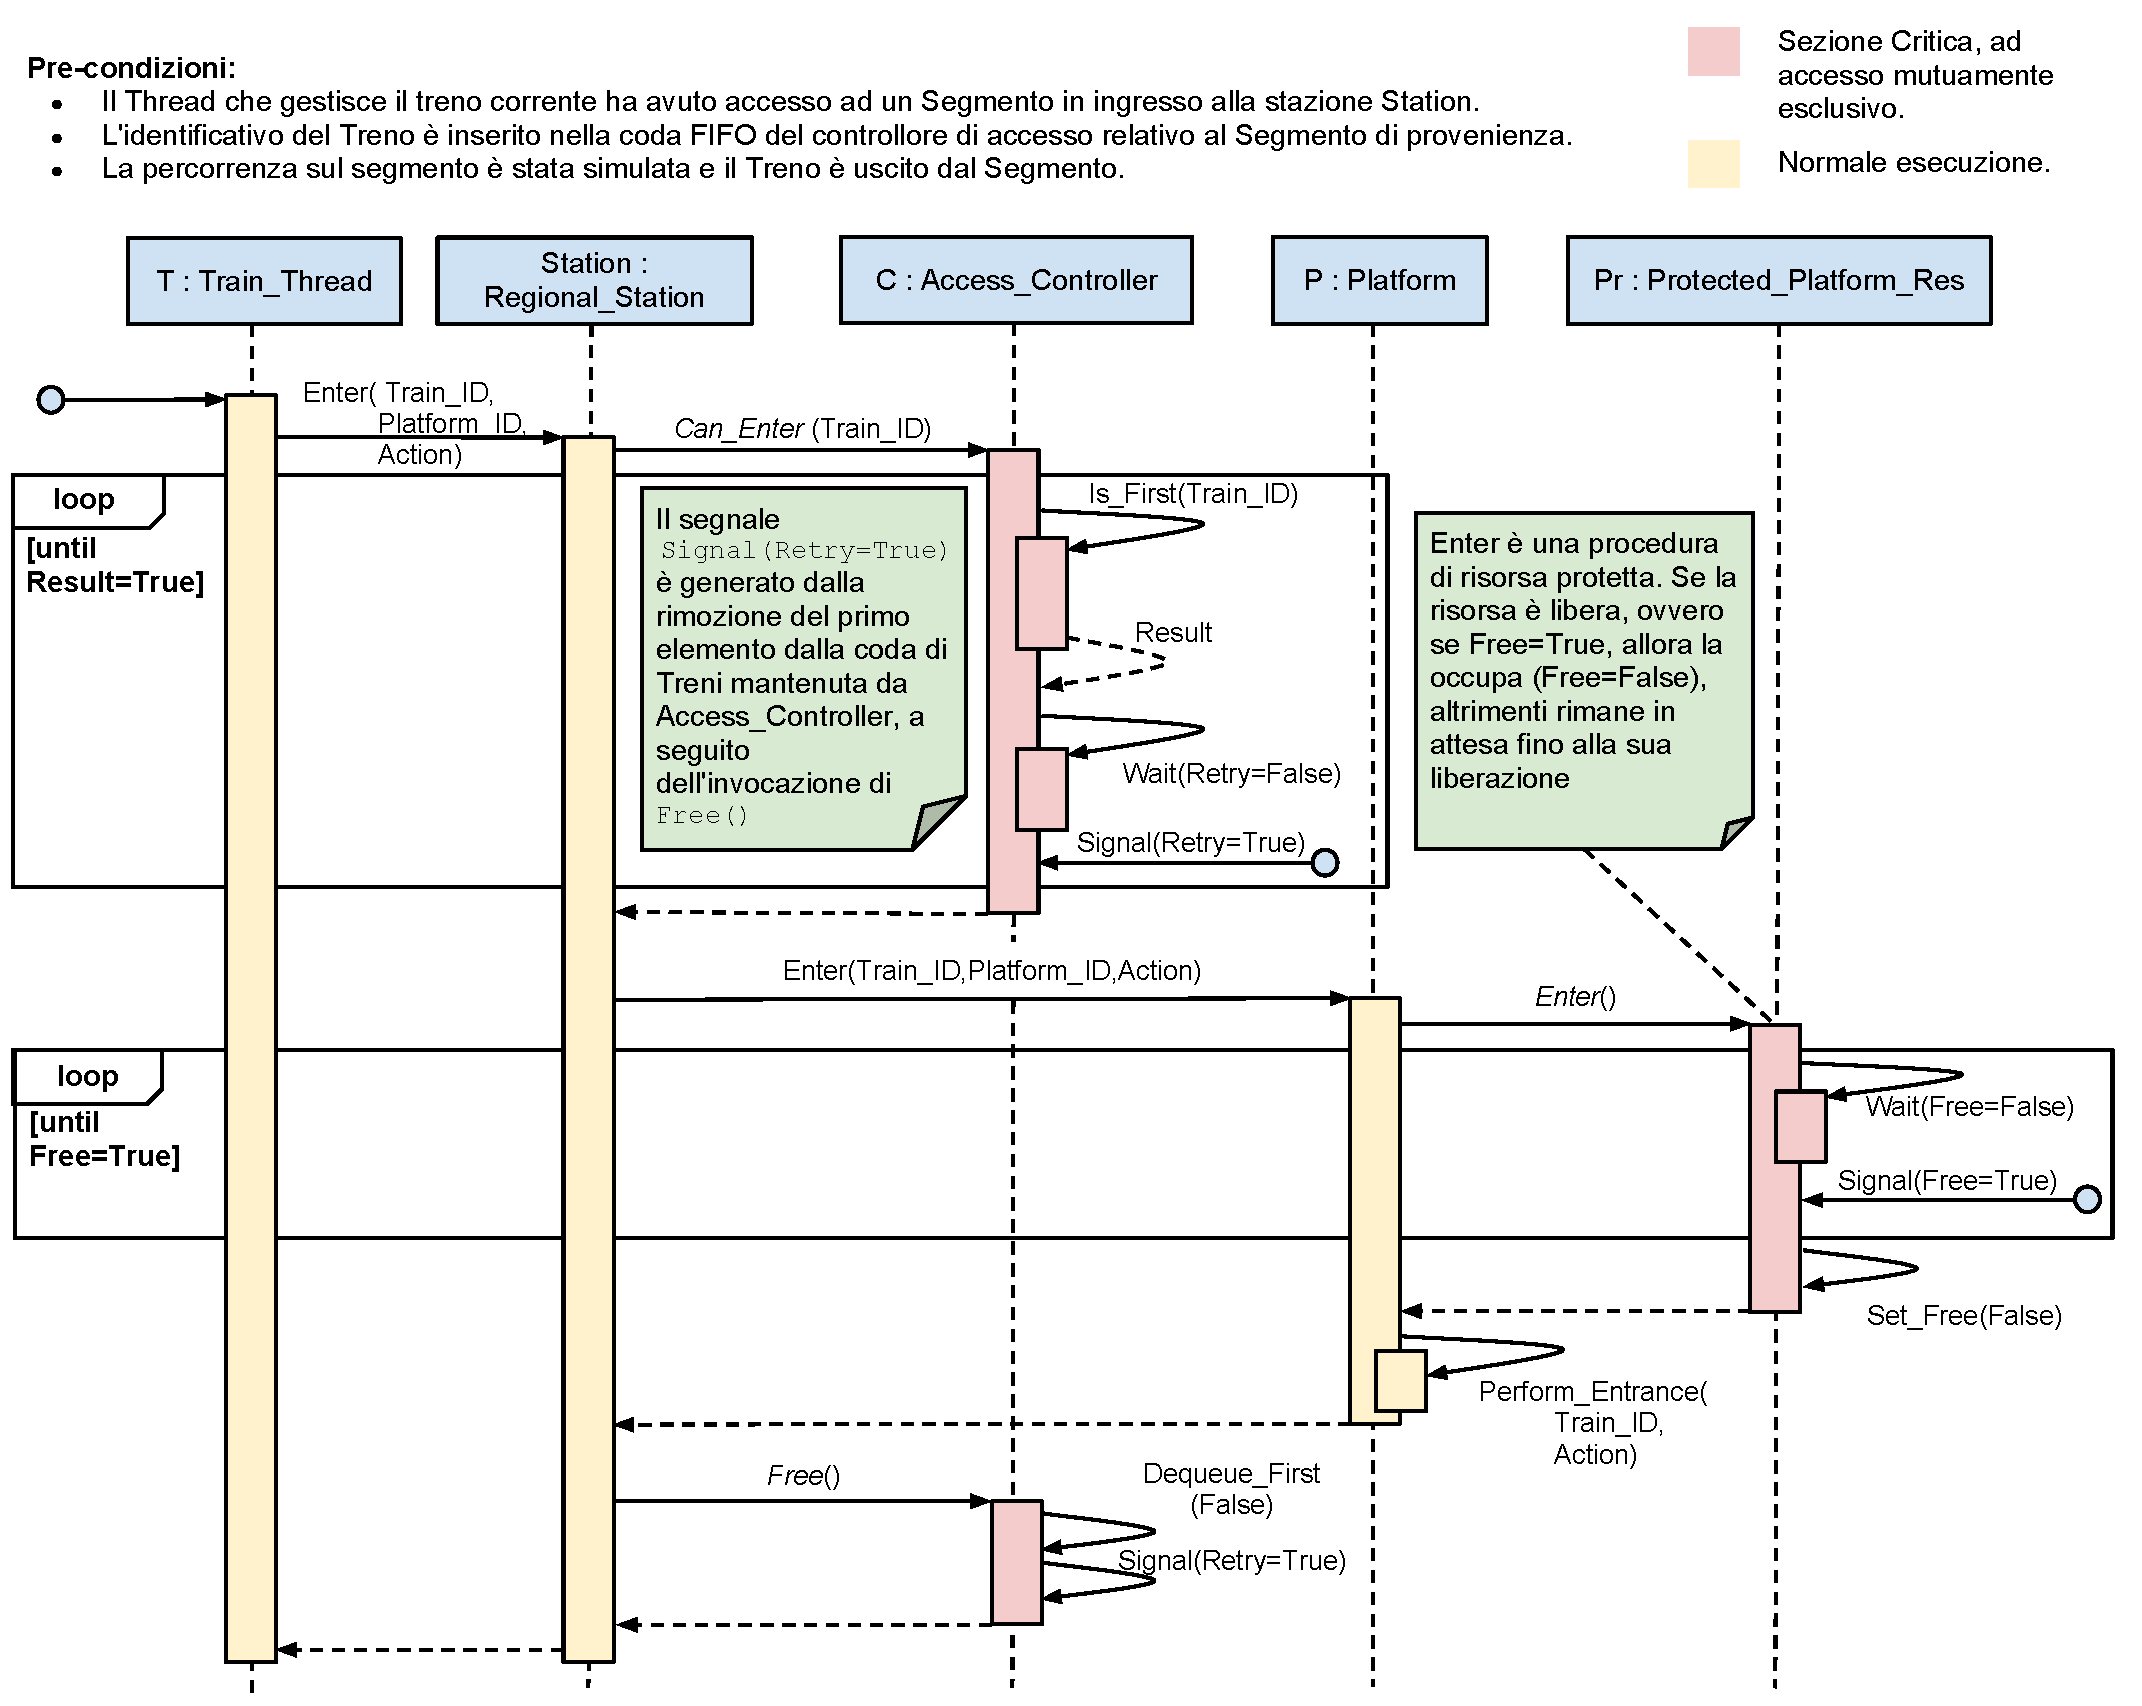
\includegraphics[trim = 45mm 0mm 0mm 0mm,scale=0.53]{imgs/platform_access_Sequence_Diagram.pdf}
			\caption{\footnotesize{Diagramma di Sequenza, operazioni necessarie per l'ingresso ad una Piattaforma.}}
			\label{fig:platform_access}
		\end{figure}
		
		I prerequisiti alla richiesta da parte di un Treno $T$ di accesso ad una Stazione sono:
		
			\begin{itemize}
				\item Il Treno $T$ ha avuto accesso ad un Segmento $S$ che collega la stazione corrente a quella dalla quale proviene. Ciò significa che il suo Descrittore sarà stato inserito nella coda \ttt{Train\_Queue} di $S$.
				\item Il Treno $T$ ha simulato la percorrenza su $S$ 
				\item Il Treno $T$ uscito dal Segmento $S$, quindi è stato rimosso dalla coda \ttt{Train\_Queue} di $S$.
			\end{itemize}
			
		Il diagramma di sequenza in figura \ref{fig:platform_access} mostra le operazioni che portano alla richiesta ordinata di accesso, e all'ingresso presso una Piattaforma.
		\begin{description}
	% ################################################# INGRESSO_ORDINATO #########################################
			\item{\ii{Ingresso Ordinato}}
		
		Per tutti i Treni provenienti dallo stesso Segmento, è necessario mantenere un ordine di richiesta di accesso alla Stazione successiva uguale a quello utilizzato per l'uscita dal Segmento. Poiché il sistema non può fare assunzioni sulle scelte dello scheduler che verrà adottato, è necessario introdurre un meccanismo che riesca a mantenere l'ordine di richiesta di accesso anche nel caso in cui, il thread che rappresenta il Treno appena uscito dal Segmento venga prerilasciato e venga eseguito il thread rappresentante il Treno successivo.

		Ho vagliato le seguenti soluzioni possibili:
		\begin{enumerate}
			\item Rappresentazione della Stazione come entità passiva ad accesso mutuamente esclusivo. Essa mantiene al suo interno una coda per Segmento, del tutto simile alla coda \ttt{Train\_Queue} interna ai Segmenti, e popolata parallelamente a \ttt{Train\_Queue}. In questo modo è semplice garantire (con un meccanismo simile a quello utilizzato per l'uscita da un Segmento) un accesso ordinato. Questa soluzione ha però uno svantaggio evidente: la richiesta di accesso avviene in mutua esclusione anche tra i Treni provenienti da Segmenti diversi, e che quindi si ritroveranno a dover superare un punto di sincronizzazione inutile, se diretti a Piattaforme diverse della Stazione.
			
			\item Una seconda possibilità prevede la presenza, all'interno di ciascuna Stazione, di una risorsa \ttt{monitor} per ciascun Segmento entrante, la quale si occuperà di garantire l'ordine di accesso (tale ordine sarà dato da una coda interna aggiornata in modo analogo alla soluzione precedentemente illustrata). Una volta che il Treno ha guadagnato il permesso di accedere in mutua esclusione alla risorsa protetta di controllo, esso avrà il permesso di interagire con la prossima Piattaforma, in modo concorrente con i Treni provenienti da altri Segmenti entranti. La coda con politica di ordinamento FIFO che indicherà l'ordine di accesso, sarà aggiornata dal Segmento mediante un'invocazione ad una procedura fornita dall'interfaccia della Stazione (ad esempio \ttt{Add\_Train}).
			In questo modo la Stazione diventerà solo un'interfaccia utilizzabile per l'accesso alle piattaforme, e inoltre i vincoli di ordinamento e accesso concorrente alle Piattaforme da Treni provenienti da Segmenti diversi saranno garantiti.
			Un esempio di pseudo-codice per il controllore di accessi è il seguente:
			
\begin{lstlisting}[label=station_access_controller]	
monitor Access_Controller
	...
	procedure Add_Train(T:Train)
	begin
		Trains_Order.Enqueue(T);
	end;

	procedure Enter(T:Train) 
	begin
		while(T.Id/=Trains_Order.First_Element()) loop
			wait(Retry_Enter);
		end loop;
	end;

	procedure Leave()
	begin
		signal_all(Retry_Enter);
	end;
end monitor;

\end{lstlisting}
			
			Lo svantaggio di utilizzare questa soluzione risiede nella creazione delle entità protette, una per ciascun Segmento entrante, che regolano l'accesso ordinato, e quindi spostano parte della conoscenza della topologia della rete ferroviaria anche sulle Stazioni, rendendone più complessa la configurazione iniziale.
			
			\item La terza soluzione esaminata e scelta, è simile alla soluzione precedente, ma a differenza di essa opera una popolazione dinamica della struttura dati che andrà a contenere le risorse protette (\ttt{Access\_Controller}) che garantiscono l'ordinamento. Ciascun Treno nell'accedere alla Stazione, includerà anche un'identificativo univoco del Segmento di provenienza, e se per esso non esisterà una controllore degli accessi, allora esso verrà creato. Questa variante ha il vantaggio per il quale le stazioni non devono necessariamente essere a conoscenza della topologia del sistema ferroviario; inoltre l'allocazione di controllori sarà limitata al massimo al numero di Segmenti in ingresso.
		\end{enumerate} 
		
		Il controllore di accessi (\ttt{Access\_Controller}) ha quindi il compito di fornire da barriera internamente alla Stazione; esso lascerà passare solamente il Treno (il thread che lo esegue) che effettivamente è primo nella coda di ordinamento.
		Siano \ttt{Enter} e \ttt{Leave} rispettivamente le due procedure protette del monitor, allora l'accesso alla Piattaforma verrà regolato nel seguente modo:
			\begin{itemize}
				\item Il Treno $T$ usa \ttt{Enter} per poter accedere alla prossima Piattaforma.
				\item Se $T$ è effettivamente il primo della Coda allora 
					\begin{itemize}
						\item prosegue all'\ii{accesso alla Piattaforma};
						\item libera l'\ttt{Access\_Controller} con \ttt{Free}. 
					\end {itemize}
				\item Altrimenti viene messo in attesa del proprio turno su una condizione (\ttt{Retry\_Enter}). I Treni in attesa sulla coda FIFO associata a questa guardia, verranno risvegliati ogni volta che un Treno effettuerà un accesso e una successiva chiamata a \ttt{Free} (la quale invocherà \ttt{signal(Retry\_Enter)} per ciascun thread in attesa).
			\end{itemize}
		
		La coda interna a ciascun \ttt{Access\_Controller} viene aggiornata nel momento in cui ciascun Treno esce dal Segmento corrispondente. 
		
	% ############################################## INGRESSO_PIATTAFORMA #########################################
		
		\item{\ii{Ingresso in una Piattaforma}}
		
		Dopo aver superato la barriera di controllo d'accesso alla Stazione \ttt{Access\_Controller}, invocando la procedura protetta \ttt{Enter}, ciascun Treno può procedere nel tentativo di ottenere l'accesso alla Piattaforma desiderata. Tale accesso avverrà quindi:
		
		\begin{itemize}
			\item In maniera sequenziale tra tutti i Treni provenienti dallo stesso segmento.
			\item In maniera concorrente tra tutti i Treni provenienti da Segmenti diversi, fornendo precedenza di accesso ai Treni di tipo \ttt{FB}.
		\end{itemize}
		
		Si rende quindi evidente la necessità di garantire l'ordine di esecuzione tra tutti i thread provenienti da uno stesso segmento, indipendentemente dalle scelte effettuate dello scheduler che verrà adottato.
		Una Piattaforma può essere modellata come un'entità che espone una interfaccia semplice, con al suo interno una struttura dati \ttt{monitor} per la regolazione dell'ordine di ingresso. A tale scopo, quest'ultima mantiene al suo interno una coda FIFO \ttt{Trains\_Order} e fornisce una procedura protetta \ttt{Add\_Train} che permette di inserirvi l'identificativo di un Treno. Questa coda manterrà non solo l'ordine di accesso tra i Treni provenienti dallo Stesso segmento, ma più in generale tra tutti i Treni che intendono accedere alla Piattaforma (può essere vista come una sorta di "prenotazione" della risorsa prima di ottenervi l'accesso). Per garatire inoltre che l'ordine di ingresso dei Treni nella coda \ttt{Trains\_Order} sia tale da fornire accesso preferenziale ai Treni di tipo \ttt{FB}, è possibile utilizzare un oggetto \ttt{Priority\_Access\_Handler} come per l'accesso al Segmento (listato \ref{priority_access_controller}), e di conseguenza prevedere il seguente comportamento per la procedura protette \ttt{Add\_Train}:
\begin{lstlisting}
	...
	procedure Add_Train(T:Train)
	begin
		Priority_Access.Gain_Access();
		Trains_Order.Enqueue(T);
		Priority_Access.Access_Gained();
		
	end;
	
\end{lstlisting}
		Una volta aggiunto l'identificativo del Treno corrente in \ttt{Trains\_Order}, può essere liberata la risorsa di controllo (\ttt{Access\_Controller}) mediante la procedura \ttt{Free} ed è quindi libero di richiedere l'accesso alla Piattaforma successiva prevista dal percorso (l'ordine di ingresso sarà rispettato). La semantica di accesso su di una Piattaforma $P$, mediante procedura di monitor \ttt{Enter} è la seguente:
		\begin{itemize}
			\item Se il Treno corrente $T$ è il prossimo a poter entrare in $P$ allora 
				\begin{itemize}
					\item Se l'azione (\ttt{action}) prevista dal Percorso è \ttt{ENTER} allora:
						\begin{itemize}
							\item esegue l'operazione di \bb{Discesa dei Viaggiatori};
							\item rilascia la risorsa, in modo tale che altri Treni possano accodarsi, e rimane in attesa fino all'orario prestabilito di partenza;
						\end{itemize}
				\end{itemize} 
			\item Se invece $T$ non è il prossimo Treno che può entrare, il Treno viene posto in attesa su variabile di condizione \ttt{Retry\_Enter}.
		\end{itemize}

Un esempio di struttura dati di controllo per una Piattaforma è visibile nel listato \ref{platform_access_controller}.

\begin{lstlisting}[label=platform_access_controller]

monitor Platform_Access_Controller 
	...
	procedure Add_Train(T:Train)
	begin
		...
	end;
	
	procedure Enter(T:Train) 
	begin
		while(T.Id/=Trains_Order.First_Element()) loop
			wait(Retry_Enter);
		end loop;
	end;
	
	procedure Leave()
	begin
		signal_all(Retry_Enter);
	end;
end monitor;
	
\end{lstlisting}
		
		L'Operazione di \bb{Discesa dei Viaggiatori}, si basa sulla possibilità che presso la Piattaforma corrente $P$ vi siano Viaggiatori all'interno della coda \ttt{Arrivals\_Queue} in attesa di un evento generato da uno specifico Treno, ovvero il suo arrivo presso $P$. L'operazione di Discesa dei passeggeri ha come precondizione l'accesso alla Piattaforma da parte di un Treno $T$ descritta in precedenza, ed è realizzata dalle seguenti azioni (eseguite dal thread associato a $T$):
		\begin{itemize}
			\item Viene estratto ciascun Viaggiatore $V$ dalla coda \ttt{Arrival\_Queue}, e per ognuno di essi:
			\begin{itemize}
				\item Se il Treno atteso da $V$ (informazione recuperabile dalla Tappa corrente del suo Biglietto) è proprio $T$ allora
					\begin{itemize}
						\item il numero di posti occupati di $T$ viene decrementato;
						\item se la Stazione corrente $S$ \bb{non} è la destinazione che $V$ deve raggiungere allora:
							\begin{itemize}
								\item l'Operazione \ttt{LEAVE} del Viaggiatore viene inserita nella coda di operazioni di \ttt{Traveler\_Pool};
								\item viene incrementato l'indice \ttt{Next\_Stage} nel Biglietto del viaggiatore $V$.
							\end{itemize}
					\end{itemize}
				\item Se $T$ invece non è il Treno atteso da $V$, quest'ultimo viene reinserito nella coda \ttt{Arrivals\_Queue}.
			\end {itemize}
		\end{itemize}
		
	Le operazioni necessarie ad attuare la Discesa dei Viaggiatori devono essere eseguite esternamente alla Sezione critica associata all'ingresso del Treno nella Piattaforma; se così non fosse infatti, essa risulterebbe occupata, e non sarebbe quindi possibile per i thread che sopraggiungono ottenere il lock sulla risorsa per eseguire \ttt{Add\_Train}.
	
	% ################################################# USCITA_PIATTAFORMA #########################################
	\item{\ii{Uscita da una Piattaforma}}

		\begin{figure}[htbp]
			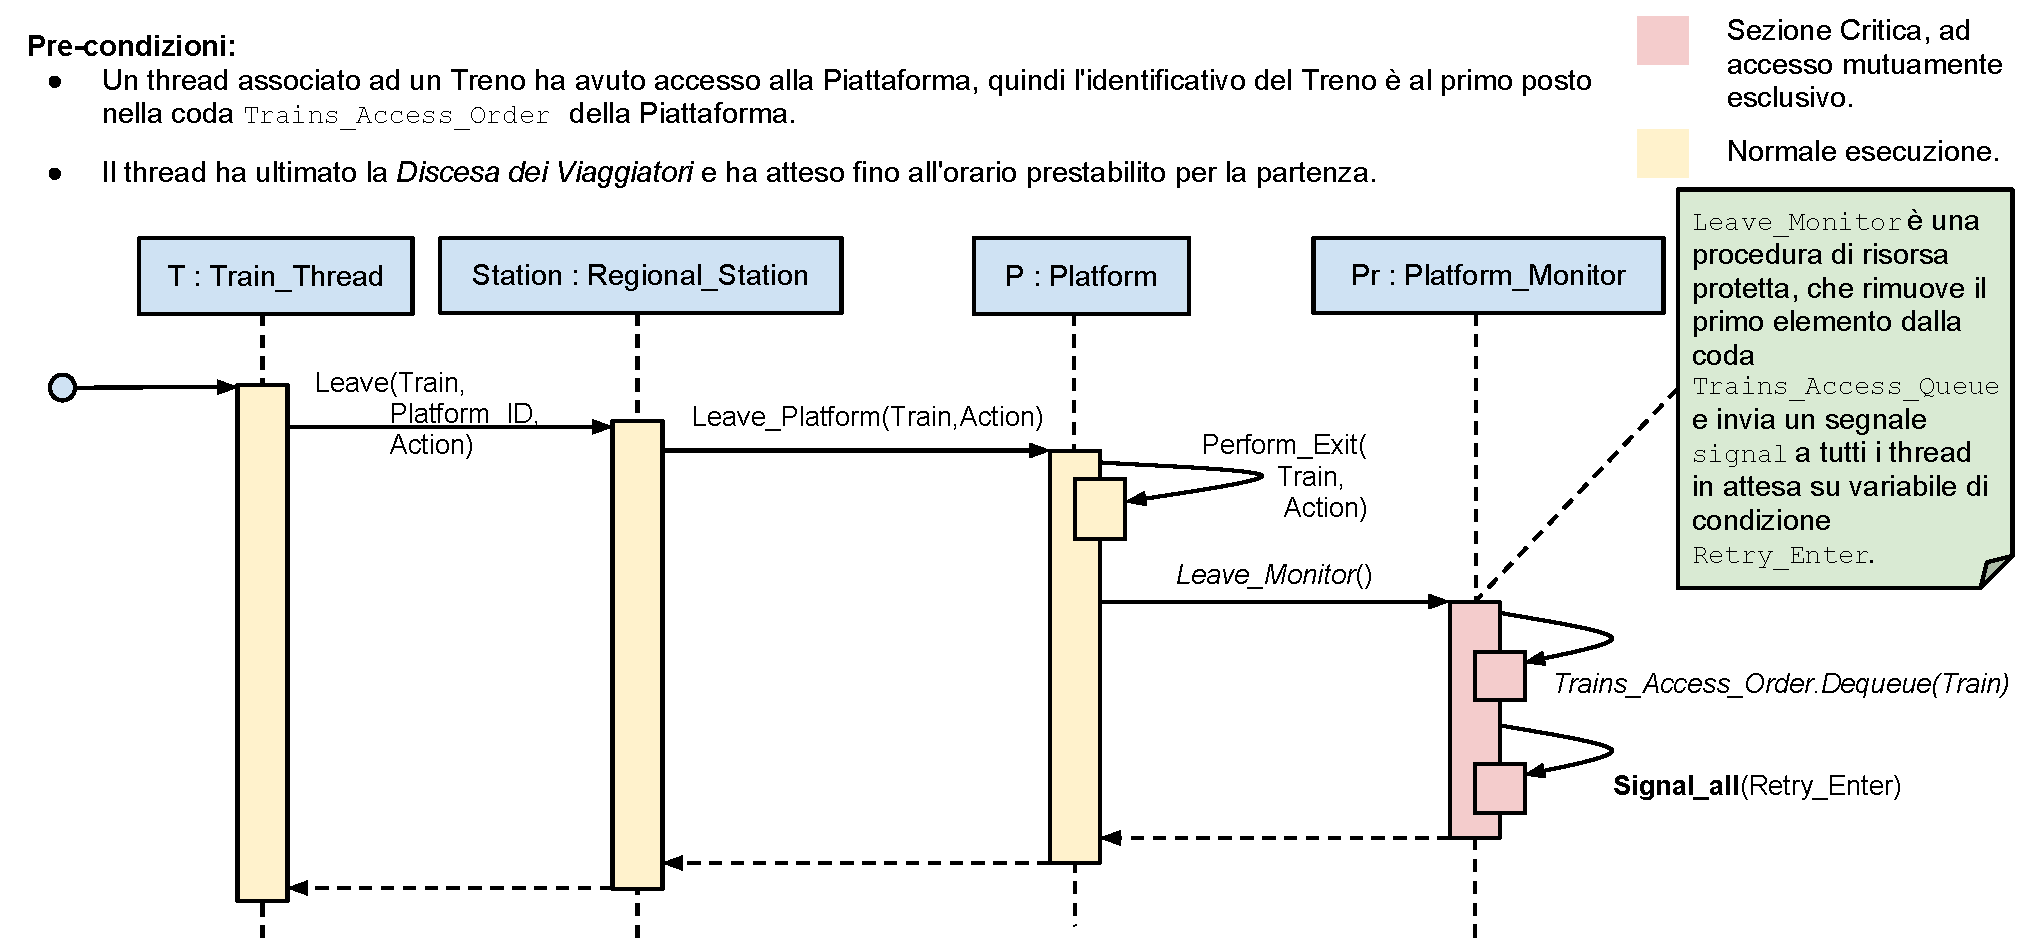
\includegraphics[trim = 45mm 0mm 0mm 0mm,scale=0.55]{imgs/platform_exit_Sequence_Diagram.pdf}
			\caption{\footnotesize{Diagramma di Sequenza, operazioni necessarie per l'uscita da una Piattaforma.}}
			\label{fig:platform_access}
		\end{figure}
		
		L'uscita da una Piattaforma $P$ necessita di due prerequisiti:
		
			\begin{itemize}
				\item Il thread che gestisce il Treno ha prima effettuato l'ingresso, e quindi il suo identificativo univoco è il primo elemento della coda \ttt{Trains\_Order} mantenuta dalla risorsa a protezione della Piattaforma.
				\item \'E già stata effettuata la Discesa dei Passeggeri (se prevista dal Percorso del Treno).
				\item \'E stato generato l'evento che notifica l'arrivo dell'orario previsto per la partenza.
			\end{itemize}
		
		A questo punto, le operazioni effettuate per completare la partenza sono:
		
			\begin{itemize}
				\item Viene effettuata la Salita dei Viaggiatori in attesa presso $P$. 
				\item Il Treno corrente registra il proprio passaggio presso la Piattaforma, memorizzando in una struttura dati apposita \ttt{Last\_Train\_Run} il proprio identificativo univoco e l'identificativo univoco della Corsa corrente \ttt{Current\_Run\_Id}.
				\item La risorsa viene rilasciata dal Treno in esecuzione mediante la procedura di monitor \ttt{Free}, la quale provvede a rimuovere il primo elemento della coda \ttt{Trains\_Order} e, se ci sono thread in attesa sulla condizione \ttt{Retry\_Enter}, a risvegliare tali thread.
			\end{itemize}
		
		La \bb{Salita dei Viaggiatori} è simile alla discesa dei Passeggeri presentata al punto precedente. Essa prevede l'esecuzione delle seguenti azioni:
		\begin{itemize}
			\item Viene estratto ciascun Viaggiatore $V$ dalla coda \ttt{Leaving\_Queue} di $P$, e per ciascuno di essi:
			\begin{itemize}
				\item Se il Treno atteso da $V$ (informazione recuperabile dalla Tappa corrente del suo Biglietto) è proprio il Treno correntemente in esecuzione $T$ e \ii{se la capienza massima di $T$ non è stata raggiunta} allora:
					\begin{itemize}
						\item il numero di posti occupati di $T$ viene incrementato;
						\item l'Operazione \ttt{ENTER} del Viaggiatore viene \ii{eseguita} a differenza di quanto avviene nella fase di Discesa dei Passeggeri: in questo modo infatti si avrà la garanzia che tutti i Viaggiatori saliti a bordo del Treno saranno in attesa nella coda \ttt{Arrival\_Queue} della Piattaforma di Stazione corretta, nel momento in cui il Treno vi accederà durante il proprio viaggio. 
					\end{itemize}
				\item Se $T$ invece non è il Treno atteso da $V$, allora viene verificato se il Treno per il quale esso è in attesa non sia già passato, qualora esso sia di tipo \ttt{FB}: per effettuare tale controllo viene acceduta la struttura dati \ttt{Last\_Train\_Run} e verificato se la corsa per la quale il Viaggiatore corrente è in attesa del Treno non sia stata già effettuata. In tal caso viene inserita l'operazione \ttt{BUY\_TICKET} per il Viaggiatore corrente nella coda di \ttt{Traveler\_Pool}, per permettere l'acquisto di un nuovo Biglietto per raggiungere la destinazione prevista a partire dalla Stazione corrente. In tutti gli altri casi, il Viaggiatore viene re-inserito nella coda \ttt{Leaving\_Queue}.
			\end {itemize}
		\end{itemize}
	\end {description}

% ############################################################################################################
% ########################################### ACCESSO_STAZIONE_GATEWAY #######################################
% ############################################################################################################		

	\subsubsection{Accesso ad una Stazione di Gateway}\label{subsubsec:gateway_stations_func}
	
	Alcuni Treni seguono percorsi che attraversano più Regioni. Tra le tappe che compongono tali percorsi, alcune indicheranno l'attraversamento di Regioni di Gateway, introdotte nella sezione \ref{sec:gateway_stations}. 
	Le azioni di Ingresso, Salita dei Viaggiatori, e Ripartenza presso questo tipo di stazioni seguono le stesse regole descritte per le stazioni Regionali nella sezione \ref{subsubsec:regional_station_access}. Esse hanno quindi un effetto locale alle Regioni (nodi) di provenienza e di destinazione.
	Per quanto riguarda invece la Discesa dei Viaggiatori, essa può prevedere un \ii{trasferimento remoto} dei Viaggiatori in attesa di arrivo.
	
	Il Passaggio di un Treno da una regione alla successiva può essere schematizzato come segue: siano $G1$ e $G2$  Stazioni di Gateway connesse, che collegano le regioni $R1$ ed $R2$, con $G1 \in R1$, e sia $G2 \in R2$. Un Percorso che attraversa i due Gateway conterrà almeno una Tappa $T1$ tale per cui il campo \ttt{next\_station} avrà il valore $G1$, \ttt{destination\_platform} una delle Piattaforme possibili per effettuare l'accesso $P$, e \ttt{region} la regione $R1$, e una tappa $T2$ tale per cui il campo \ttt{next\_station} avrà il valore $G2$, \ttt{destination\_platform} la stessa piattaforma specificata in $T$, e \ttt{region} la regione $R2$.
	Le operazioni eseguite saranno le seguenti:
	\begin{itemize}
		\item Il Treno corrente $T$ effettua l'accesso alla Stazione $G1$, Piattaforma $P$.
		
		\item $T$, se previsto dal Percorso, effettua Discesa dei Viaggiatori. Tale azione è simile alla Discesa descritta in sezione \ref{subsubsec:regional_station_access}, ma se un Viaggiatore una volta sceso proseguirà il proprio percorso su un nodo diverso da quello corrente, esso verrà trasferito mediante messaggio remoto al nodo successivo, e solo a questo punto verrà inserita l'Operazione \ttt{ENTER} del Viaggiatore nella coda di operazioni di \ttt{Traveler\_Pool} locale al nodo destinazione.
		
		\item Il descrittore del Treno corrente $D_T$ viene serializzato (\ii{marshalling}), e inviato tramite invocazione remota alla Stazione di Gateway della Regione $G2$ ad essa connessa. L'individuazione dell'indirizzo della regione specificata nel parametro \ttt{region}, avviene interrogando il \ttt{Name\_Server}, se esso non è già presente in una cache locale.
		\item Il flusso ciclico di istruzioni eseguite dal thread che gestisce $T$ viene interrotto (esso potrà così ottenere un nuovo Descrittore di Treno ed eseguire per esso le proprie operazioni).
		\item Presso la regione $R2$, stazione di Gateway $G2$, vengono eseguite le seguenti operazioni:
			\begin{itemize}
				\item Il Descrittore viene de-serializzato (\ii{unmarshalling}).
				\item I dati del Descrittore $D_{T'}$ presenti nella regione $R2$ vengono aggiornati con quelli ricevuti.
				\item Viene aggiunto l'identificativo di $T$ nella coda \ttt{Trains\_Order} della Piattaforma $P$.
				\item Vengono operate attesa fino all'orario di partenza previsto (secondo il clock del nodo corrente), Salita dei Viaggiatori e Partenza dalla Stazione come per le Stazioni Regionali.
				\item Viene restituito un messaggio di \ii{acknowledgement} al nodo $R1$, che comunica l'avvenuta esecuzione delle operazioni.
			\end{itemize}
		\item Una volta ricevuto il messaggio di \ii{acknowledgement}, presso il nodo $R1$, viene liberata la piattaforma corrente (viene rimosso il primo elemento della coda \ttt{Trains\_Order}) in modo tale da permettere ad altri Treni di occuparla.
	\end{itemize}
	
	Ciò che garantisce la correttezza della soluzione presentata, relativamente a discesa e salita dei passeggeri locale, è la modalità con la quale il Viaggiatore viene accodato presso la Stazione di Gateway come descritto nella sezione \ref{subsec:percorrenza_viaggiatore}, ovvero in modo tale per cui:
	\begin{itemize}
		\item Presso le coda \ttt{Arrival\_Queue} delle Piattaforme nel nodo di partenza vi saranno tutti e soli i passeggeri in attesa di scendere presso la Stazione di Gateway, se previsto dal loro Biglietto.
		\item Presso le code \ttt{Leaving\_Queue} delle Piattaforme nel nodo di destinazione vi saranno invece solamente i Viaggiatori che vogliono raggiungere una destinazione interna al nodo corrente.
	\end{itemize}  
	Si noti che la soluzione riportata prevede lo scambio di due messaggi remoti, il primo per la transizione del Treni tra le Regioni, e il secondo di acknowledgement per poter liberare la risorsa Piattaforma presso il nodo di partenza. Di fatto, data l'inaffidabilità della rete, è possibile che uno dei due messaggi scambiati non venga ricevuto dal nodo di destinazione. Abbiamo quindi due casi:
		\begin{itemize}
			\item \ii{L'invio del primo messaggio fallisce.} In questo caso, il flusso di esecuzione del thread che gestisce il Treno viene interrotto. Per semplicità si può pensare che il Treno sia cancellato a causa di un guasto, o si può ridurre il Percorso fino alla Tappa che ha causato l'errore, dopo essersi accertati dell'effettiva irraggiungibilità del nodo destinazione.
			\item \ii{Il messaggio di acknowledgement non viene consegnato.} In questo caso il problema è più grave. Il Treno presso il nodo di destinazione continua la propria corsa, mentre la Piattaforma abbandonata rimane occupata, e quindi inutilizzabile dai Treni che sopraggiungono. Per risolvere questo tipo di problema è possibile prevedere un tempo massimo di occupazione della Piattaforma, oltre il quale richiedere l'effettivo stato di occupazione della Piattaforma presso la Stazione di Gateway della Regione di destinazione e, nel caso in cui risultasse libera, procedere alla liberazione della stessa, impostando \ttt{Free} a \ttt{True}. 
		\end{itemize}
	 
	
